% This is a sample document using the University of Minnesota, Morris, Computer Science
% Senior Seminar modification of the ACM sig-alternate style. Much of this content is taken
% directly from the ACM sample document illustrating the use of the sig-alternate class. Certain
% parts that we never use have been removed to simplify the example, and a few additional
% components have been added.

% See https://github.com/UMM-CSci/Senior_seminar_templates for more info and to make
% suggestions and corrections.

\documentclass{sig-alternate}
\usepackage{color}
\usepackage[colorinlistoftodos]{todonotes}

%%%%% Uncomment the following line and comment out the previous one
%%%%% to remove all comments
%%%%% NOTE: comments still occupy a line even if invisible;
%%%%% Don't write them as a separate paragraph
%\newcommand{\mycomment}[1]{}

\begin{document}

% --- Author Metadata here ---
%%% REMEMBER TO CHANGE THE SEMESTER AND YEAR AS NEEDED
\conferenceinfo{UMM CSci Senior Seminar Conference, April 2019}{Morris, MN}

\title{An Analysis of IoT System Applications on Global Public Health Issues}

\numberofauthors{1}

\author{
% The command \alignauthor (no curly braces needed) should
% precede each author name, affiliation/snail-mail address and
% e-mail address. Additionally, tag each line of
% affiliation/address with \affaddr, and tag the
% e-mail address with \email.
\alignauthor
David Chong\\
	\affaddr{Division of Science and Mathematics}\\
	\affaddr{University of Minnesota, Morris}\\
	\affaddr{Morris, Minnesota, USA 56267}\\
	\email{chong050@morris.umn.edu}
}

\maketitle
\begin{abstract}
In this paper I detail information needed in order to understand an Internet of Things (IoT) system. I then examine researchers efforts in designing systems to detect potentially problematic mosquito populations. I then examine security concerns from the perspective of designing a resilient smart home.
\end{abstract}

\keywords{Internet of Things}

\section{Introduction}
\label{sec:introduction}

The Internet of Things is a frequent topic of interest in the Computer Science discipline; but it is often talked about in vague terms. I will be detailing what is an IoT system, what goals IoT systems have, how those goals can be met, and some concerns that come up when discussing IoT systems.
% Not really happy with this part

I will be analyzing a few real world use cases of IoT systems. I will discuss differences between the systems and why certain requirements are needed in some while not in others.

\section{Background}
\label{sec:background}

%Here I need to talk about hardware acceleration, algorithms and big O, auto vectorize and parallel computing and threading
%May briefly talk about various IoT devices like Intel Edison, Particle Photon, and Raspberry Pi

\subsection{Algorithms}
\label{sec:algorithms}

% Here I need to cover big O in order to analyze pseudocode later on
This is quite a verbose topic so I will only be dipping our toes on this subject in order to later explain efficiency of a program in a meaningful way. When looking at a program we can think of each command as a step. Each step can be measured using big O. Big O is used to measure the run time of a function in terms of n -- the number of passes required to complete a computation. This measurement can be linear, quadratic, logarithmic, etc. This important to consider when needing to optimize the efficiency of a program.

\subsection{Systems}
\label{sec:systems}

% Here I need to cover auto-vectorize, parallel computing and threading
Parallel computing is a valuable asset when designing a system. Use of parallel computing allows the system to perform multiple processes at the same time. Internet of Things devices may need to process vast amounts of data. Usage of parallel computing, and more specifically automatic vectorization lends way to more efficient systems. Automatic vectorization can be thought of as performing multiple steps at once. Consider a for loop that iterates one by one and computes a simple addition problem then sets that value equal to a unique variable. Automatic vectorization would allow for a defined number of those iterations to be performed simultaneously. One can imagine four steps happening at once.

\subsection{Hardware Acceleration}
\label{sec:acceleration}

% Here I need to cover hardware acceleration
When designing a system one must consider the hardware they will be using to implement said system. If possible, hardware acceleration can be used in order to have a system work more efficiently. It does this by using hardware like a computer's graphics card in order to process information rather than leaving all the work to the CPU. This is important later on as a system I will cover has the goal of being both efficient computationally and power consumption wise.

\subsection{Cryptography}
\label{sec:cryptography}

% Here I might talk about symmetric key cryptography as it is mentioned in both the secure data provenance and IoT security challenges articles

\subsection{Devices and IoT structure}
\label{sec:devices}

% Here I need to cover the different devices so that people understand later on when they are mentioned

Some of the devices used in the implementation of IoT systems include: Raspberry Pi 3, Intel Edison, cellular phones, etc. Any internet connected device can be considered an IoT device so keep in mind this list is far from exhaustive. The specifications of each device can vary greatly in terms of CPU clock speeds, system memory, flash memory, voltage requirements, and more. All these factors and more must be considered when designing an IoT system.

IoT is made up of three layers: preception, network and application. The preception layer includes the physical devices which collect information from various other devices in order to then send that information to the network layer. The network layer is the connection between the preception and application layers. The application layer takes the information from the network layer and processes it in a way that is likely valuable to an end user.

These devices are able to communicate using various methods such as RFID, NFC, Bluetooth, WIFI, and more. Each method of communication has its own various specifications such as frequency and range. Some of these methods are available on devices while others are not so that must be considered when designing an IoT system.

% Talk about cloud computing and providers
% Talk about Iaas, PaaS, SaaS

\section{Example A: Mosquito Detection - an IoT system}
\label{sec:mosquito}

In our first example, Ravi et al. were able to design an IoT system that was able to detect mosquito populations with an 80\% accuracy. There were able to achieve this using tiny board computers like Intel Edison and Raspberry Pi 3. Their main goal was to create a system that would be able to detect mosquito populations more efficiently than current methods. More granular goals included: keeping cost per device low, maintain high efficiency through various optimizations -- this in turn creates another goal of maintaining low power usage in order to not need to service remote devices.

The researchers needed to first decide which devices would best suit their application. The main deciding factor here was how long the battery would last as the devices are meant to be used in remote locations such as mines, swamps, etc.

%Here I am going to add possibly figure 2 (Need to explain FFT, kNN, and bayesian classifier at least briefly) and definitely figure 3 from the mosquito article.

\begin{figure}
\centering
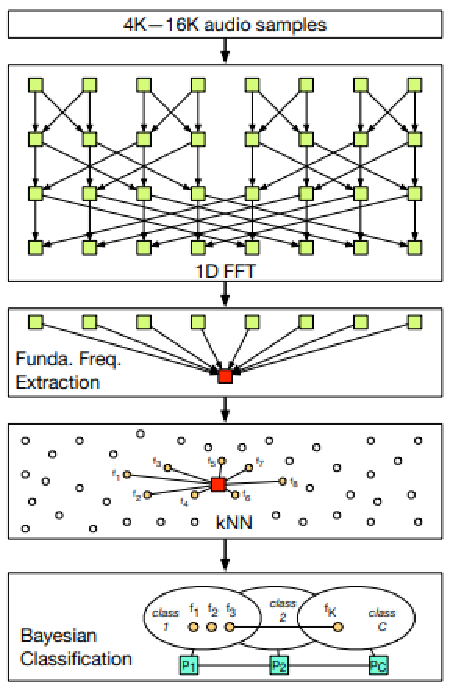
\psfig{file=imagetopdf1.pdf,width =3in}
\caption{High-Level View of the Computational Flow of Insect Classification}
\label{fig:singleColumnFigure1}
\end{figure}

The previous figure give us a view of how data is processed in order to get meaningful data from the mosquito measurements. Each sample must be processed through the three steps in order to accurately classify and code the data. The researchers found this embedded computation method to be 80 times more energy efficient than using radio communication of the raw data. This method provides around two months of usage versus the radio methods mere 20 hours on a 2000 mAh AA battery on an Intel Edison. It is worth mentioning here -- the system sends data once per day and remains in a low power standby when not computing or sending data.

%Here I want to analyze the big O for the pseudocode

\begin{figure*}
\centering
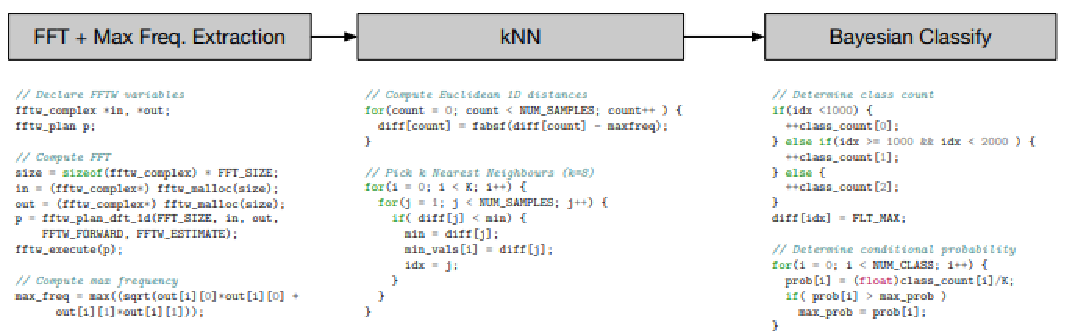
\psfig{file=imagetopdf2.pdf,width =5.3in}
\caption{Pseudocode Sketches of the Underlying Algorithm and Arithmetic}
\label{fig:twoColumnFigure1}
\end{figure*}

The researchers were able to identify that 80-90\% of the runtime was taken up by the FFT component -- see above figure. They were able to determine that usage of hardware accelerators were able to speed up the computation of this step by a factor of two.

The researchers also found that a trade off between precision and power usage would be valuable to the system. Originally their implementation used 32 bit floating-point hardware. This meant that computation on this data would be slower and require more storage -- both of these factors reduce the overall energy efficiency of the device. This prompted the researchers to instead choose to use 16 bit fixed point as their primary data type. They determined that this trade off would be worth the loss in precision in this specific case.

The researchers found they were able to add flags to their code in order to further optimize compilation. An example of this would be use of the -msse2 flag. This allows the code to auto-vectorize and run parts in parallel. %this needs to be better explained
Other optimizations such as loop unrolling, reassociation and other arithmetic transformations due to use of compiler flags allow for further trade offs to be made granting higher speed of computation and less energy usage while losing precision. The researches found this acceptable with the caveat that overall classification accuracy remained unaffected.

These optimizations are both made on the hardware and the software.

%Here I want to import figure 6 from the mosquito article -- un-opt has no flags, opt1 has single threading, opt2 has multithreading - need to talk about hardware optimizations

\begin{figure}
\centering
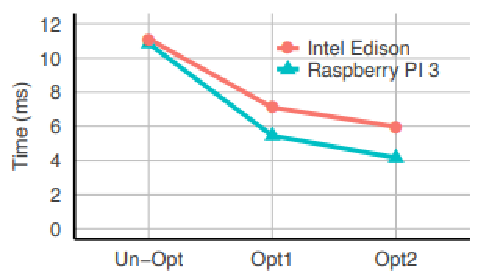
\psfig{file=imagetopdf3.pdf,width =3in}
\caption{Impact of Hardware and Software Optimizations on Performance}
\label{fig:singleColumnFigure2}
\end{figure}

%Need to explain FFT, kNN, and bayesian classifier at least briefly or above - needed in order to talk about software optimizations
%Will summarize the figures here rather than show

\begin{figure}
\centering
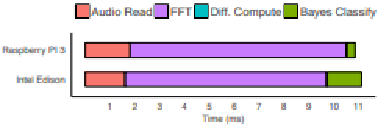
\psfig{file=imagetopdf4.pdf,width =3in}
\caption{Performance Runtime Breakdown of Different Compute Stages of the Classifier}
\label{fig:singleColumnFigure2}
\end{figure}

In the end; the researchers were able to design a system which they say could be used in tandem with existing insect classification efforts in order to provide a more rich set of data to help identify the problematic mosquito populations quickly.

\section{Example B: Resilient Smart Home - IoT security}
\label{sec:home}

% Talk about issues that can arise in IoT systems and their causes
% Internet is unavailable
% Note this is very rough and needs to be cleaned up

It is important to consider how one would go about designing an IoT system that is resilient. It is not out of the realm of possibility that a system could lose connection to the internet due to any number of causes.

Causes for internet outage: technical problems, natural causes, targeted attacks. All of these lend way to possible negative effects such as lack of service, possibly providing an attack window on the system, or allowing unauthorized access. It is also important to note that a system may need manual intervention in order to run properly after an outage occurs. All of these reasons point to a need for resilient IoT systems, especially in cases where safety is a main concern. One of the articles I read in preparation for this paper details several functions that may be used in IoT systems in order to provide a more resilient system. These functions include: the ability to detect cloud failure, providing a notification, or performing a service transfer. This list is far from exhaustive but provides an idea of possible solutions available to help aid the resilience issue.

When designing an IoT system it is important to identify services provided which one would consider essential. We must design around these essential services in order to provide acceptable service in case of external failure such as internet disconnection.

The earlier that security is considered when designing a IoT system the better. Security issues can quickly snowball out of control especially with certain IoT systems as they could be designed to be easily scalable. If the issue is unfound and deployed to a wide audience it is difficult address after the fact as the initial problem becomes obscured over time. It is also possible that issues may lie within the hardware or software creating another layer of obscurity in terms of identifying root security flaws.

While tamper and fault resistance are not mandatory in terms of functionality of an IoT system they are still important to consider as each layer of defense makes attacks on the system more difficult to carry out. Network attacks that take advantage of computational phenomena such as instance cache attacks, timing attacks, and faults induced by the Row hammer approach are all possible and must be considered when designing an IoT system.

As IoT grows as a fairly new idea we must consider the vast amount of data, some of which can be sensitive, making IoT systems lucrative targets to cybercriminals. The systems running these devices can be limited making security requirements difficult to manage.

Main challenges: authentication, data integrity, data provenance, privacy, and access control. These devices are sometimes deployed remotely so physical security of the device must also be noted. This means that security against both physical and network attacks must be designed for.

% Talk about physical unclonable functions (PUFs) and how they ensure data provenance

\section*{Acknowledgments}
\label{sec:acknowledgments}

I would like to thank professors Lamberty and Machkasova for there countinuous help and feedback throughout this course. I would like to thank the other professors in the CSCI faculty as well. I would also like to thank my friends and family who have helped me through the process of my Senior Seminar.

% The following two commands are all you need in the
% initial runs of your .tex file to
% produce the bibliography for the citations in your paper.
\bibliographystyle{abbrv}
% sample_paper.bib is the name of the BibTex file containing the
% bibliography entries. Note that you *don't* include the .bib ending here.
\bibliography{sample_paper}
% You must have a proper ".bib" file
% and remember to run:
% latex bibtex latex latex
% to resolve all references

\end{document}